\section{Positivstellensätze without denominators}

Let $X=(X_1,\ldots,X_n)$ be indeterminates and $n \in \N$. Consider the basic semi-algebraic set $\{g \ge 0\}$ given by $g =(g_1,\ldots,g_s) \in \R[X]^s$.  The template questions of this chapter are: Does the condition $f > 0$ on $\{g \ge 0\}$ imply that $f \in \cP(g)$? Can one use another set rather than $\cP(g)$ in such a context? We'll see positive answers in a number of situations and provide links to linear and semidefinite programming.
The presentation in this chapter is based on \cite{averkov2013constructive}.

%\subsection{Affine version of Farkas lemma}

%Recall that $\blue{\cone(M)}$ is the convex conic hull of \blue{$M$}. One of the basic Nichtnegativstellens\"atze without denominators is the Farkas lemma. Its affine version can be formulated as follows.
%We say that a polynomial is linear if its degree is at most one. 
%
%\begin{lemma}[Affine version of Farkas lemma]
%	\label{lem:farkas}
%	Let $f,a_1,\ldots,a_m \in \R[X]$ be $n$-variate linear polynomials, and let the polyhedron $K = \{a_1 \ge 0,\ldots a_m \ge 0\} \subseteq \R^n$ be non-empty.
%	Then the following conditions are equivalent:
%	\begin{enumerate}[(i)]
%		\item $f \ge 0$ on $K$
%		\item $f \in \cone(1,a_1,\ldots,a_m)$. 
%	\end{enumerate}
%\end{lemma}
%\begin{proof}
%	Exercise
%\end{proof}


\subsection{P\'olya: a positivstellensatz on a simplex}

The templates for the following results will be: if $f > 0$ on a compact set $K$, then there exists some algebraic representation of $f$ providing the evidence that $f \ge 0$ on $K$. So, you see that it is not a characterization, but an implication: you require strict positivity and have the evidence for non-negativity only. Such results can of course be converted into a characterization of positivity. It suffices to invoke the above implication for $f - \eps$ in place of $f$, where $\eps>0$ is small enough so that $f - \eps$ is still positive on $K$. 


The following theorem is about homogeneous polynomials, which are positive on the standard simplex.
For dealing with exponent vectors of homogeneous polynomials, we introduce the notation 
\[
	\bE^n_d := \setcond{\alpha \in \Z_+^n}{|\alpha | =d}.
\]
We also use the notation $\alpha ! = \alpha_1 ! \cdot \ldots \cdot \alpha_n !$ for $\alpha = (\alpha_1,\ldots,\alpha_n) \in \Z^n_+$.


\begin{theorem}[P\'olya 1928] 
	Let $f \in \R[X]$ be a homogeneous polynomial, with $f> 0$ on the simplex 
	\[
		\Delta := \setcond{(x_1,\ldots,x_n) \in \R_+^n}{x_1 + \cdots + x_n =1}.
	\]
	Then there exists $N \in \Z_+$ such that all coefficients of $(X_1 + \cdots + X_n)^N f(X)$ are non-negative. 
\end{theorem}
\begin{proof}

	We write $f$ as $\sum_{\alpha \in \bE^n_d} c_\alpha X^\alpha$. The expression $(X_1 + \cdots + X_n)^N$ can be expanded so that we get
	\begin{align*}
		 g & := (X_1+ \cdots + X_n)^N f 
		 \\ & = \sum_{\beta \in \bE^n_N} \frac{N!}{\beta !} X^\beta \sum_{\alpha \in \bE^n_d} c_\alpha X^\alpha 
		 \\ & = \sum_{\alpha \in \bE^n_d, \beta \in \bE^n_N} c_\alpha \frac{N!}{\beta!} X^{\alpha+\beta}.
	\end{align*}
	
	We see that $g$ is a homogeneous polynomial of degree $d+N$:
	\[
		g = \sum_{\gamma \in \bE^n_{d+N}} A_\gamma X^\gamma
	\]
	whose coefficients can be expressed through the coefficients of $f$ by:
	\begin{equation}
		\label{A:gamma:first:eq}
		A_\gamma = \sum_{\alpha \in \bE^n_d \,:\, \alpha \le \gamma} c_\alpha \frac{N!}{(\gamma-\alpha)!} .
	\end{equation}
	We want to analyze the behavior of $A_\gamma$ for growing $N$. To this end, we factor out an appropriate term in the above sum describing $A_\gamma$:
	\[
		A_\gamma = \frac{N!(N+d)^d}{\gamma!} \sum_{\alpha \in \bE^n_d \, : \alpha \le \gamma} c_\alpha \frac{\gamma !}{(\gamma-\alpha)! (N+d)^d}.
	\]
	In the latter sum, the coefficients $c_\alpha$ are multiplied by values depending on $N$. In order to see how these values behave for $N \to \infty$, we express them differently. Since both $\gamma!$ and $(\gamma-\alpha)!$ are products of $n$ factorials and since $|\alpha|=d$, we get
	\[
		\frac{\gamma!}{(\gamma-\alpha)! (N+d)^d} = \prod_{i=1}^n \frac{\gamma_i !}{(\gamma_i-\alpha_i)! (N+d)^{\alpha_i}} ,
	\]
	where $\alpha = (\alpha_1,\ldots,\alpha_n)$ and $\gamma=(\gamma_1,\ldots,\gamma_n)$. The quotient $\gamma_i! / (\gamma_i-\alpha_i)!$ is the product of the $\alpha_i$ many values $\gamma_i-\alpha_i+1,\ldots,\gamma_i$. Hence 
	
	\[
		\frac{\gamma_i !}{(\gamma_i-\alpha_i)! (N+d)^{\alpha_i}} = \left(\frac{\gamma_i - \alpha_i+1}{N+d} \right) \cdots \left( \frac{\gamma_i}{N+d} \right).
	\]
	Summarizing this gives
	\[
		A_\gamma = \frac{N!(N+d)^d}{\gamma!} \sum_{\alpha \in \bE^n_d \, : \alpha \le \gamma} c_\alpha \prod_{i=1}^n \left(\frac{\gamma_i - \alpha_i+1}{N+d} \right) \cdots \left( \frac{\gamma_i}{N+d} \right).
	\]
	We can discard the condition $\alpha \le \gamma$  and let the sum go over all $\alpha \in \bE^n_d$, for if $\alpha_i > \gamma_i$ for some $i \in [n]$, then the respective term in the product occurring in the latter representation of $A_\gamma$ is equal to zero. 
	
	In this context, it will be convenient to use the notation
	\[
		(x)_t^m := x (x-t) \cdots x (x - (m-1) t).
	\]
	Note that for $t \to 0$, $(x)_t^m \to x^m$, so for small $t$, the value $(x)_t^m$ is a perturbed version of $x^m$. In this notation $A_\gamma$ can be represented as
	
	\[
		A_\gamma = \frac{N!(N+d)^d}{\gamma!} \sum_{\alpha \in \bE^n_d} c_\alpha \left(\frac{\gamma_1}{N+d} \right)_{1/(N+d)}^{\alpha_1} \cdots  \left(\frac{\gamma_n}{N+d} \right)_{1/(N+d)}^{\alpha_n}.
	\]	
	Since one has $|\gamma|= N+d$, we get $\gamma / (N+d) \in \Delta$. Consider the polynomial
	
	\[
		f_t(X) = \sum_{\alpha \in \bE^n_d} c_\alpha (X_1)_t^{\alpha_1} \cdots (X_n)_t^{\alpha_n}.
	\]
	
	The polynomial function $f_t(x)$ converges to $f(x)$ uniformly on $\Delta$ as $t \rightarrow 0$ (recall that the uniform and the pointwise convergence are equivalent for continuous functions on a compact set). Thus, \blue{by our assumption that $f > 0$ on $\Delta$}, we get $f_t(x)>0$ for all $x \in \Delta$ if $t$ is small enough. Up to a positive multiple, our $A_\gamma$ coincides with $f_t(\gamma/ (N+d))$ for $t=\frac{1}{N+d}$. It follows that $A_\gamma  > 0$ for all $\gamma$, if $N$ is large enough. 
\end{proof}

\begin{remark}
\blue{
The proof above shows that for large enough $N$ every possible monomial $X^\gamma$, for $\gamma \in \bE^n_{d+N}$, appears in $(X_1 + \dots + X_n)^N f(X)$ with a positive coefficient.}

\blue{As an example consider the polynomial $f = X^2 - 2 X Y + 2 Y^2 = (X - Y)^2 + Y^2$ which is positive on~$\Delta \subseteq \R^2$.
We have
\[
(X+Y)^4 f(X) = X^6 + 2 X^5Y + 5 X^2Y^4 + 6 XY^5 + 2Y^6,
\]
in which every coefficient is non-negative, but not every monomial of degree six appears.
However, in $(X+Y)^6 f(X)$ every monomial of degree six appears and has a positive coefficient.
}
\end{remark}

\begin{remark}
	Quantitative aspects of P\'olya's theorem (how large is $N$, depending on $f$) were investigated by Reznick \& Powers \cite{Powers:Reznick:2001}. They give a choice of $N$ depending on $d,n$ and $\min_{x \in \Delta} f(x)$. Their paper also contains a complete proof of P\'olya's theorem. 
\end{remark}

\subsection{P\'olya's theorem and copositivity} 

A symmetric matrix $A \in \cS^n$ is called co-positive if $\sprod{x}{A x} \ge 0$ holds for all $x \in \R_{\ge 0}^n$. This means the quadratic polynomial $f(x) = \sprod{x}{A x}$ is non-negative on the standard simplex $\Delta$. If $\sprod{x}{Ax}>0$ holds for all $x \ne 0$, then $A$ is called strictly copositive and the corresponding quadratic polynomial $f(x)$ is strictly positive on the standard simplex. P\'olyas theorem addresses strict positivity as a special case. Checking whether a matrix is copositive (strictly copositive) is hard. This can also be seen from the fact that a number of NP-hard problems can be formulated as conic problems over the copositive cone (conic problems will be the topic of Chapter~\ref{conic:optimization}; roughly, a conic program is a problem of optimization of a linear objective function over an affine slice of a given cone). See also the survey \cite{dur2010copositive}. Copositive programming is a special case of inequality constrained quadratic programming. 


\subsection{P\'olya's theorem and the cone of homogeneous polynomials} 

Let's denote by $\oP_{n,d}(\Delta)$ the closed convex cone of all homogeneous $n$-variate polynomials of degree $d$ that are non-negative on the simplex $\Delta$. P\'olyas theorem provides a sequence of polyhedral cones $\oP_{n,d}^N(\Delta)$ approximating the cone $\oP_{n,d}(\Delta)$ arbitrarily well, as $N \to \infty$. In fact, the condition that all coefficients of $(X_1+\cdots +X_n)^N f$ are non-negative is a system of linear inequalities for the coefficients of $f$. The polynomial $f$ occurs linearly in the expression $(X_1+\cdots + X_n)^N f$, or to put it a bit differently, the map $f \mapsto (X_1+ \cdots +X_n)^N f$ is linear. For $N=0$, the condition is just that all coefficients of $f$ are non-negative. Thus, for $N=0$, the set $\oP_{n,d}^N(\Delta)$ is just a simplicial cone. For large $N$ explicit inequalities on the coefficients of $f$ can be found in the proof. By \eqref{A:gamma:first:eq}, the inequalities are 
	\begin{align*}
		\sum_{\alpha \in \bE^n_d \,:\, \alpha \le \gamma} c_\alpha \frac{1}{(\gamma-\alpha)!} & \ge 0 & & \forall \gamma \in \bE^n_{N+d}.
	\end{align*}


\begin{example}
	To illustrate this, we consider approximations of the copositive cone for $n=2$.  We consider a quadratic form $f(x,y)$ given as $f(x,y) = a x^2 +  b x y + c y^2$. So, in this case $\oP_{n,d}(\Delta)= \oP_{2,2}(\Delta)$ is a three-dimensional cone. It will be more convenient for us to look at the slices of the cone and so we fix a normalization \blue{$2 a + b + 2 c = 2$} of coefficients of $f$, which corresponds to slicing $\oP_{2,2}(\Delta)$ by a hyperplane (the slice by the hyperplane $a + b + c=1$ is unbounded, see Exercise~\ref{ex:polya:unboundedslice} below). It is known, and \blue{sketched in Exercise~\ref{ex:polya:P22decomposition} below}, that the cone $\oP_{2,2}(\Delta)$ is generated by the polynomial $xy$ and the PSD quadratic forms (that is, each $f\in \oP_{2,2}(\Delta)$ is $f = \alpha g + \beta xy$, where $\alpha, \beta \ge 0$ and $g$ is PSD). Note that $f$ is PSD if and only if $a \ge 0, c \ge 0, a c - (\frac{b}{2})^2 \ge 0$ holds (this is a basic fact in linear algebra). We look at the equality $a c - (\frac{b}{2})^2 =0$ which, in view of $2a + b + 2c = 2$, can be formulated as $a c - (1- (a+c))^2 = 0$. This equation describes an ellipse tangent to the $a$ and $c$ axes and lying in the non-negative orthant. 
	
	The best is to write the condition in $a+c$ and $a -c$. Using $\xi=a+c$ and $\eta = a-c$ and multiplying by $4$, this can be formulated as
	\[
		\xi^2 - \eta^2 - 4 (1- \xi)^2 = 0.
	\]
	This is
	\[
		- 3 \xi^2  + 8 \xi - 4 - \eta^2 = 0
	\]
	which gives
	\[
		3 \xi^2 - 8 \xi + 4 + \eta^2 = 0
	\]
	and can be written as
	\[
		3 (\xi - 4/3)^2 + \eta^2 = \frac{4}{3}.
	\]
	So we get an equation of the ellipse (that is, the boundary of the PSD forms sliced by $2a + b + 2c = 2$ is an ellipse). We remark that from $a c - (1 - (a+c))^2 = 0$ one gets $a \ge 0$ and $c \ge 0$. Furthermore both $a =0$ and $c=0$ are possible (by choosing $a=0, c=1$ and $a=1, c = 0$). Here is a picture of it generated with WolframAlpha:
	\begin{center}
		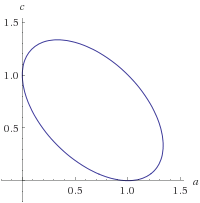
\includegraphics[width=150pt]{sdp_ellipse}
	\end{center}
	
	\blue{The full slice of $\oP_{2,2}(\Delta)$ is then given by the convex hull of this ellipse and the origin, which can be seen by scaling a general form $\alpha g + \beta xy$ back to the chosen hyperplane $2a + b + 2c = 2$.}
	Here is a picture, generated by Benjamin Peters using Matlab that shows how (the slices of) $\oP_{2,2}^N(\Delta)$ approximate (the slice of) $\oP_{2,2}(\Delta)$.
	
	\begin{center}
	\begin{tikzpicture}[]
	\pgftext{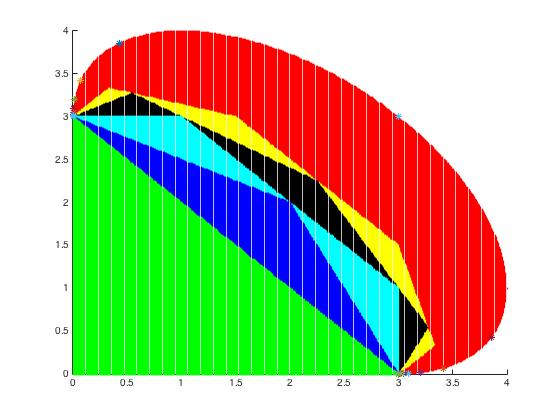
\includegraphics[width=150pt]{polya_polyhedra}} at (0pt,0pt);
	\end{tikzpicture}
	\end{center}

	As $N$ grows, $\oP_{2,2}^N(\Delta)$ is growing larger and larger so that every interior point of the red region is eventually covered. But for some of these points it takes very long to be covered. 
\end{example}

\begin{exercise}
	\label{ex:polya:unboundedslice}
	Show that the slice of 
	\[
		\oP_{2,2}(\Delta) := \setcond{(a,b,c) \in \R^3}{f:=a x^2 + b x y + c y^2 \ge 0  \ \text{on} \ \Delta}
	\] 
	by the hyperplane $a+b+c=1$ is unbounded. 
\end{exercise}
\begin{solution}
	Clearly, the slice is non-empty, because all $(a,b,c)$ with $a + b + c=1$ and $a,b,c \ge 0$ are in the slice. It suffices to find $(a',b',c') \in \oP_{2,2}(\Delta)$ with $a' + b' +c'=0$. Adding arbitrary non-negative multiples of this to any point of the slice we do not fall out of the slice. This shows that a slice contains a ray and so is unbounded. As we know from the convexity theorem, unboundedness of a closed convex set can always be certified by providing a ray that is contained in the set. Finding such an element is easy: $(x-y)^2 = x^2 - 2xy + y^2$ is non-negative ant it yields $a'=1, b'=-2$ and $c'=1$. Done!
\end{solution}

%\begin{exercise*}
%	 Determine all hyperplane slices of $P_{2,2}(\Delta)$ which are non-empty and bounded. UNDER CONSTRUCTION: At this point the exercise may come too early as duality of cones has not been discussed, yet. 
%\end{exercise*}
%\begin{solution}
%	psd quadratic forms are in $P_{2,2}(\Delta)$ and $xy$ is also in $P_{2,2}(\Delta)$. This allows to see that $P_{2,2}(\Delta)$ is the sum of two cones $K_1 + K_2$, where $K_1$ are quadratic forms with non-negative coefficients and $K_2$ are psd quadratic forms. So if slicing $K_1$ or $K_2$, we get an unbounded set, we have unboundedness. One can also show the converse, if both slice of $K_1$ and slice of $K_2$ is bounded, then also the slice of $K_1 + K_2$ will be bounded (standard convexity). 
%	UNDER CONSTRUCTION
%\end{solution}

\begin{exercise}
	\label{ex:polya:P22decomposition}
Show that $\oP_{2,2}(\Delta)$ is the convex conic hull of all psd quadratic forms $q(x,y)$ and the polynomials $xy$.
\end{exercise}

\begin{solution}	
(Sketch of the solution)
%
Clearly, the mentioned convex conic hull is a subset of $\oP_{2,2}(\Delta)$. To prove the converse, it suffices to show that every point on an extremal ray of $\oP_{2,2}(\Delta)$ is psd quadratic form or coincides with $xy$ up to a multiple. Note that $\oP_{2,2}(\Delta)$ is pointed and full-dimensional. Every point $f$ on the extremal ray is on the boundary ans so has a zero in $\Delta$. If it has a zero in the relative interior of $\Delta$ it is a square and so a psd form. If it has a zero in an endpoint of $\Delta$, there are the following cases. If both endpoints are zeros of $f$, then $f$ coincides with $xy$ up to a non-negative multiple. If only one endpoint is zero, then we tweak on $f$ so that it remains non-negative on $\Delta$ using $x^2$ or $y^2$. This shows that $f$ is not extremal.
\end{solution}


\subsection{Handelman: a positivstellensatz on a polytope} 

P\'olya's theorem can be used to derive a positivstellensatz on polytopes.

For $a_1,\ldots,a_m \in \R[X]$ and $a=(a_1,\ldots,a_m)$ we introduce the semiring generated by $a$ as 
\[
	\cS(a) := \setcond{\sum_{e=(e_1,\ldots,e_m) \in E} c_e a_1^{e_1} \cdots a_m^{e_m} }{c_e \in \R_{\ge 0} \ \forall e \in E, \ E \subseteq \Z_+^m \ \text{finite}}.
\]
The set $\cS(a)$ consists of conic combinations of products of powers of $a_1,\ldots,a_m$. It is clear, that a representation of $f$ as an element of $\cS(a)$ gives a certificate for non-negativity of $f$ on $\{a \ge 0\}$. 

\begin{remark}[P\'olya on general simplices]
P\'olya's theorem applied in a straightforward way yields a positivstellensatz on an arbitrary simplex. If $a_1,\ldots,a_{n+1}$ are linear polynomials and $S:=\{a_1 \ge 0,\ldots, a_{n+1} \ge 0\}$ is an $n$-dimensional simplex, then every polynomial $f$ strictly positive on $S$ belongs to $\cS(a)$. The sketch of the argument is as follows. Up to rescaling, one can assume $a_1 + \cdots + a_{n+1} = 1$. The original variables $X_1,\ldots,X_n$ can be expressed through $a_1,\ldots,a_{n+1}$, which will become our `new variables', and if $f$ has degree at most $d$, we can replace each monomial in~$f$ by a homogeneous polynomial of degree $d$ in `new variables' $a_1,\ldots,a_{n+1}$. After this, applying P\'olya's theorem, we get the desired conclusion. 
\end{remark}

\blue{We need two ingredients to extend P\'{o}lya's result to arbitrary polytopes.
For the first, let }$f \in \R[X]$ be a polynomial of degree at most $d$ and let~$l \in \R[X]$ be a linear homogeneous polynomial.
Then, $g = l^d f (X/l)$ is a polynomial, too. Moreover, $g$ is a homogeneous polynomial and we call it a \emph{homogenization} of $f$ with respect to $l$.

Let's see an example for how this kind of homogenization works. If  say $f = X_1 + X_1 X_2 + X_1 X_2 X_3^2$ and $l=X_1 + X_2 +X_3$, then the degree of $f$ is $4$. There is a monomial of degree one and a monomial of degree two. We multiply each of these monomials by an appropriate power of $l$ to get the homogeneous polynomial
\[
	g = X_1 l^3 + X_1 X_2 l^2 + X_1 X_2 X_3^2. 
\]

\blue{The second ingredient is one of the basic Nichtnegativstellens\"atze without denominators -- the Farkas lemma.
Recall that $\cone(M)$ is the convex conic hull of $M$.
We say that a polynomial is linear if its degree is at most one.}
%
\blue{\begin{lemma}[Affine version of Farkas lemma]
	\label{lem:farkas}
	Let $f,a_1,\ldots,a_m \in \R[X]$ be $n$-variate linear polynomials, and let the polyhedron $K = \{a_1 \ge 0,\ldots, a_m \ge 0\} \subseteq \R^n$ be non-empty.
	Then, the following conditions are equivalent:
	\begin{enumerate}[(i)]
		\item $f \ge 0$ on $K$
		\item $f \in \cone(1,a_1,\ldots,a_m)$. 
	\end{enumerate}
\end{lemma}
\begin{proof}
	Exercise
\end{proof}
}

\begin{theorem}[Positivstellensatz of Handelman]
	Let $a = (a_1,\ldots,a_m) \in \R[X]^m$ be polynomials of degree at most one and let the polyhedron $S:= \{a \ge 0\}$ defined by the inequalities $a \ge 0$ be non-empty and bounded. Then every polynomial $f \in \R[X]$ strictly positive on $S$ belongs to $\cS(a)$. 
\end{theorem}
\begin{proof}
	Without loss of generality, we can assume that $S \subseteq \R_{\ge 0}^n$ (because we can translate $S$ into the non-negative orthant $\R_{\ge 0}^n$, and translation is just an affine change of coordinates in the space $\R^n$). 
	
	Every polynomial is bounded on \blue{the compact set} $S$ so that the polynomial $X_1 + \cdots + X_n + a_1(X) + \cdots +a_m(X)$ has an upper bound $t \in \R_{> 0}$ on $S$. Let 
	\[
		q = t - (X_1 + \cdots + X_n) - (a_1(X) + \cdots + a_m(X)).
	\] 
	By construction $q \ge 0$ on $S$. We introduce new indeterminates $Y = (Y_1,\ldots,Y_m)$ and $Z$ and the polynomials 
	\[
		\sigma = \frac{1}{t} ( X_1 + \cdots + X_n + Y_1 + \cdots +Y_m + Z)
	\]
	and
	\[
		g = f(X) + c \sum_{i=1}^m (a_i(X) - Y_i)^2
	\]
	in these indeterminates. Here, $c \in \R_{>0}$ is a constant that will be fixed in what follows. 
	
	Let $\Delta$ be the simplex given by 
	\[
		\Delta:=\setcond{(x,y,z) \in \R_{\ge 0}^{n+m+1}}{\sigma(x,y,z) = 1}.
	\]
	The $\Delta$ is up to rescaling a standard simplex (and so it is as good as a standard simplex for our purposes).
	Let $A$ be the subset of $\Delta$ given by 
	\[
		A = \setcond{(x,y,z) \in \Delta}{a_i(x) = y_i \ \forall i \in [m]}.
	\]
	The polynomials $f$ and $g$ coincide on $A$ and \blue{$a_i(x) = y_i \geq 0$, for all $i \in [m]$ on~$A$.
	Hence, $f = g > 0$ on $A$.} Above, we've lifted our~$f$ to a polynomial $g$ in a larger space and in that larger space, the positivity of~$f$ on the original set $S$ is translated to the positivity of $g$ on $A$. 
	
	Since $\blue{g} > 0$ on $A$, $\blue{g}$ is also positive on a small compact neighborhood of $A$. In $\Delta$ and outside this small neighborhood, $g$ can be made arbitrarily large, by choosing $c>0$ sufficiently large. Indeed, if we are away from $A$, the sum occurring in the definition of $g$ can be bounded from below by a positive constant and so, choosing the factor $c$ in the definition of $c$ sufficiently large we can ensure that $g> 0$ on the whole $\Delta$. Clearly, one can construct a homogeneous polynomial $g_0$ such that $g=g_0$ on $\Delta$: Just homogenize $g$ with respect to $\sigma$, by setting $g_0 := \sigma^{\deg g} g( X / \sigma, Y / \sigma, Z / \sigma)$. 
	
	Applying P\'olya's theorem to $g_0$, we get that for some large enough integer $N \in \Z_+$ all coefficients of $\sigma^N(X,Y,Z) g_0(X,Y,Z) $ are non-negative. Substituting $Z = t - (X_1 + \cdots + X_n) - (Y_1 + \cdots + Y_m)$, the polynomial $\sigma$ is turned to $1$. Subsequent substitutions $Y_i = a_i(X)$, turn the polynomial $g$ to $f$. We thus, conclude that
	$f = g_0(X,a_1(X),\ldots,a_m(X), q(X))$ is in the semiring  \[
		\cS(X_1,\ldots,X_m,a_1(X),\ldots,a_m(X),q(X)).
	\] Note that $X_1,\ldots,X_m, q(X)$ do not contribute to this semiring, because by Farkas' lemma (Lemma~\ref{lem:farkas}), these polynomials of degree at most $1$ are in $\cone(1,a_1,\ldots,a_m)$. This shows that the latter semiring coincides with $\cS(a)$. So, the assertion follows.
\end{proof}


\subsection{Handelman's theorem and linear programming}

Let's borrow the notation $a=(a_1,\ldots,a_m)$ and $S$ of Handelman's theorem and let $f \in \R[X]$ be arbitrary. In view of Handelman's theorem, the polynomial optimization problem
\[
	\min \setcond{f(x)}{a \ge 0}
\]
over the polytope $S= \{a \ge 0\}$ has the dual formulation 
\[
	\max \setcond{y \in \R}{f - y \ge 0  \ \text{on} \ S} = \sup \setcond{y \in \R}{f - y \in \cS(a)}.
\]
We really need to pass to the supremum, because Handelman's theorem is a positivstellensatz (it is about `strict' positivity). Now we can modify this problem by replacing the whole $\cS(a)$ by its truncated version
\[
	\cS_E (a) := \setcond{ \sum_{e \in E} c_e a^{e_1} \cdots a^{e_m}}{c_e \ge 0 \ \forall e \in E} \,,
\]
where $E \subseteq \Z_+^m$ is finite and fixed. The problems
\begin{equation}
	\label{handelman:relaxation}
	\max \setcond{y}{f - y \in \cS_E(a)}
\end{equation}
give lower bounds on the original minimization problem. In view of Handelman's theorem, the hierarchy of such problems with, say, $E=E^m_d$ and $d \in \N$ gives optimal values that converge to the optimal value of the original problem, as $d$ grows. Unfortunately, the convergence may be quite slow (because Handelman is based on P\'olya and so it inherits the convergence problems of P\'olya).

Let's also note that \eqref{handelman:relaxation} is a \emph{linear} problem. The objective is linear (it's just one variable $y$). The constraint $f -y \in \cS_E(a)$ is the linear equality system 
\[
	 y+ \sum_{e=(e_1,\ldots,e_m) \in E} c_e a_1^{e_1} \cdots a_m^{e_m} = f
\]
for the decision variable $y \in \R$ and the non-negative decision variables $c_e \in \R_{\ge 0}$. Indeed, the $c_e$'s and $y$ occur linearly in this expression. The polynomial $f$ is the right hand side. 

\begin{remark}
	Applicability of Handelman-based approaches (including analysis of convergence etc.) has been discussed in several sources. 
\end{remark}

\subsection{Quadratic modules and constrained polynomial optimization} 

\label{quadr:modules:pop}

If $a=(a_1,\ldots,a_s) \in \R[X]^s$ are arbitrary polynomials, then the set 
\[
	\cM(a):= \setcond{g_0 + g_1 a_1 + \cdots + g_s a_s}{g_0,\ldots,g_s \ \text{are SOS} }
\]
is called the quadratic module generated by $a=(a_1,\ldots,a_s)$. Thus, the general constrained polynomial optimization problem, \blue{with objective function $f \in \R[X]$,}
\begin{equation}
	\label{constr:pop}
	\inf \setcond{f(x)}{x \in \R^n, a_1(x) \ge 0,\ldots, a_s(x) \ge 0}
\end{equation}
over the set $\{a \ge 0\}$
can be relaxed to
\begin{equation}
	\label{module:relax}
	\sup \setcond{y \in \R}{f - y\in \cM(a)}.
\end{equation}
In fact, the supremum is a lower bound on the infimum, because the elements of $\cM(a)$ are non-negative on $\{a \ge 0\}$. The condition $f - y \in \cM(a)$ can be formulated as a semidefinite constraint. For this purpose it will be convenient to introduce the family $\cS^\infty$ of infinite-size symmetric matrices with only finitely many non-zero entries. For such matrices $A \in \cS^\infty$ the PSD property can be defined in the usual way. So, we also have a PSD cone $\cS_+^\infty$ in that space. Let 
\[
	m(X) = (X^\alpha)_{\alpha \in \Z_+^n}
\] 
be the infinite vector containing all possible monomials $X^\alpha$. 

A polynomial $g$ is SOS if and only if $g=m(X)^\top Z m(X)$, where $Z = (z_{\alpha,\beta})_{\alpha,\beta \in \Z_+^n}$ is PSD. Thus, the condition $f - y \in \cM(a)$ can be written as 

\begin{equation}
 f(X) - y = m(X)^\top Z_0 m(X) + \sum_{j=1}^s a_j(X) m(X)^\top Z_j m(X),
 \label{eq:quadr:mod:conditions}
\end{equation} 
where $Z_0,\ldots,Z_s \in \cS_+^\infty$ are infinite PSD matrices, whose entries are indexed by exponent vectors $\alpha = (\alpha_1,\ldots,\alpha_n) \in \Z_+^n$. Thus, our relaxed problem \eqref{module:relax} is the infinite SDP
\begin{equation}
	\label{inf:sdp}
	\sup \setcond{y \in \R}{Z_0,\ldots,Z_s \in \cS_+^\infty, \ y + m(X)^\top Z_0 m(X) + \sum_{j=1}^s a_j(X) m(X)^\top Z_j m(X) =f(X)} \,.
\end{equation}
The latter problem can be modified to a finite problem, since $\cS_+^\infty$ essentially contains $\cS_+^k$ for every $k$. That is, the latter problem can be truncated to the problem 
\begin{equation}
	\label{trunc:module:realax}
	\sup \setcond{y \in \R}{Z_0,\ldots,Z_s \in \cS_+^k, \ y + m_d(X)^\top Z_0 m_d(X) + \sum_{j=1}^s a_j(X) m_d(X)^\top Z_j m_d(X) = f(X)},
\end{equation}
where $m_d(X) = (X^\alpha)_{\alpha \in E_d^n}$, $d \in \N$ \blue{and $k = |E^n_d|$}. It is clear that the optimal value of~\eqref{trunc:module:realax} is a lower bound on the optimal value of~\eqref{inf:sdp} and one can approximate the optimum of \eqref{inf:sdp} arbitrarily well by choosing $d$ sufficiently large.

In what follows we try to establish cases of equivalence of \eqref{constr:pop} and \eqref{module:relax} by deriving positivstellensätze that are based on quadratic modules. 

\begin{remark}[What kind of certificate should we prefer?]
	So far, we've seen several sets used for certifying positivity and leading to various relaxations of polynomial optimization. The sets are 
	\begin{itemize}
		\item the semiring $\cS(a)$ (used in Handelman's theorem when the $a_j$'s are linear),
		\item the quadratic module $\cM(a)$ (introduced above),
		\item the preordering $\cP(a)$ (can also be used just in the same way as $\cM(a)$ was used above). 
	\end{itemize}
	Which of them can one use? Which of them are the better ones? As for the first question, there is a guarantee of convergence of the respective hierarchies if we have established a respective stellensatz (though, convergence may be really slow). As for the second question, comparison of such sets is not an obvious matter. Assume that $f>0$ on $\{a \ge 0\}$ and we can certify non-negativity of $f$ on $\{a \ge 0\}$ by representing it as an element of $\cM(a)$ and also by representing it as an element of $\cP(a)$. Will the representation as an element of $\cM(a)$ be shorter? This is not really clear! Note that both representations would involve SOS-polynomials and we do not know much about their degrees. 
\end{remark}


\subsection{Positivstellensätze involving quadratic modules}

In this section, we'll see that quadratic modules yield positivstellens\"atze on bounded sets, if we add an additional special polynomial to the generators of the underlying quadratic module. As a consequence, we'll also see that the assertion of Handelman's theorem remains true if we replace $\cS(a)$ by $\cM(a)$. 

\begin{exercise}
	\label{prop:prod:pm:product}
	Show the following: Let $X_1,\ldots,X_n,Y_1,\ldots,Y_n$ be indeterminates. Let $E_+^n$ and $E_-^n$, respectively, be the set of all vectors $e \in \{-1,1\}^n$ with an even resp. odd number of entries equal to $-1$. Then 
	\[
		X_1 \cdot \ldots \cdot X_n \pm Y_1 \cdot \ldots \cdot Y_n = \frac{1}{2^{n-1}} \sum_{e \in E_\pm^n} \prod_{i=1}^n (X_i + e_i Y_i).
	\]
	In particular, $X_1 \cdot \ldots \cdot X_n \pm Y_1 \cdot \ldots \cdot Y_n$ belong to the semiring generated by $X_1+Y_1,\ldots,X_n+Y_n,X_1 - Y_1,\ldots,X_n-Y_n$. 
\end{exercise}
\begin{solution}
	Induction on $n$. 
\end{solution}

\begin{lemma} \label{lem:t:minus:squares}
	Let $f \in \R[X] = \R[X_1,\ldots,X_n]$ and let $\rho > 0$. Then, there exists $t \in \R$ such that $t + f$ and $t- f$ belong \blue{to $\cP(\rho - \|X\|^2)$, that is, }to the preordering generated by $\rho - \|X\|^2 = \rho - (X_1^2 + \cdots + X_n^2)$. 
\end{lemma}
\begin{proof} 
\blue{Write $f = \sum_\alpha c_\alpha X^\alpha$.}
	We use $t = \sum_\alpha |c_\alpha| (\rho+1)^{|\alpha|}$. Since the definition of $t$ does not depend on changing $f$ to $-f$ (because $|c_\alpha| = |-c_\alpha|$), it suffices to check the assertion for $t + f$. We have 
	\[
		t+ f = \sum_\alpha |c_\alpha| ( (\rho+1)^{|\alpha|} + \sign(c_\alpha) X^\alpha) .
	\]
	\blue{If $\alpha = 0$, then the corresponding term in $t+f$ is $|c_0|(\rho+1+\sign(c_0)) \geq 0$.}
	For $\alpha \ne 0$, we apply Exercise~\ref{prop:prod:pm:product} to  $(\rho+1)^{|\alpha|} \pm X^\alpha$ and conclude that $t+f$ is in the semiring generated by all $\rho+1 \pm X_i$ with $i \in [n]$. Now, it suffices to see that $\rho+1 \pm X_i$ is in the preordering generated by $\rho - \|X\|^2$. Due to the symmetry we can assume $i=1$. Since changing $X_1$ to $-X_1$ does not change $\|X\|^2$, it suffices to look at $\rho + 1 + X_1$. We have
	\[
		\rho+1 + X_1 = \frac{1}{2} \bigl( (\rho+1) + (1+X_1)^2 + X_2^2 + \cdots + X_n^2  + (\rho - \|X\|^2) \bigr) \,.\qedhere
	\]
\end{proof}
%
\blue{Observe that, if $t \in \R$ is a valid choice in Lemma~\ref{lem:t:minus:squares}, then every $\bar t \geq t$ also satisfies $\bar t \pm f \in \cP(\rho - \|X\|^2)$.}
%
The following lemma will be applied in the case $\{a \ge 0 \} \subseteq B$ by choosing $B$ to be a large box. 
\begin{lemma} \label{lem:transfer}
	Let $a=(a_1,\ldots,a_s) \in \R[X]^s$ and let $f \in \R[X]$ be strictly positive on $\{a \ge 0\}$. Let $B \subseteq \R^n$ be compact. Then there exists $g \in \cM(a)$ such that $f - g $ is strictly positive on $B$. 
\end{lemma}
\begin{proof}
	The set \blue{$a(B):= \setcond{\left(a_1(x),\ldots,a_s(x)\right)}{x \in B} \subseteq \R^s$ is the image of a continuous function of a compact set, and is thus compact.}
	So there exists \blue{$\gamma > 0$} with $a(B) \subseteq (-\infty, 2 \gamma]^s$. Consider $T:= \setcond{x \in B}{f(x) \le 0}$. Since $f> 0$ on \blue{the closed set} $\{a \ge 0\}$, we get $a(T) \cap [-2 \eps, 2 \gamma]^s = \emptyset$ for a sufficiently small $\eps>0$. This can also be formulated as the inequality $f(x) > 0$ being fulfilled for all $x \in B$ satisfying $a_i(x) \ge -2 \eps$ for all $i \in [s]$. We now introduce the univariate polynomial $h(t) := t \left( \frac{t - \gamma}{\gamma + \eps} \right)^{2N}$, where $N \in \N$. On $[0,2\gamma]$, the polynomial \blue{$h$} is small for large $N$. In fact, on $[0,2\gamma]$, we have $0 \le h(t) \le \blue{2} \gamma (\gamma / (\gamma+\eps))^{2N}=:c(N)$. On the other hand, when $t \le - 2 \eps$, then $h(t)$ is negative and $|h(t)|$ is big: we have $- h (t) \ge 2 \eps ((\gamma + 2 \eps)/ (\gamma+\eps))^{2N}=:C(N)$.
	
	We now plug the $a_j$'s into $h$ and take the sum, obtaining $g(X) := \sum_{j=1}^s h(a_j(X))$. For $x \in B$, in the case $a_j(x) \ge - 2 \eps$ for all $j \in [s]$, the terms $h(a_j(x))$ with $a_j(x) \ge 0$ are small and the terms $h(a_j(x))$ with $a_j(x) \le 0$ are negative. Thus, if $N$ is large enough, we get $f(x) - g(x) > 0$. Whenever there exists $a_j(x) \le - 2 \eps$, the term $-h(a_j(x))$ is large, while the terms $h(a_j(x))$ for $a_j(x) \ge - 2 \eps$ are either negative or small. Hence $f(x) - g(x) > 0$ also in the case of having $j$ with $a_j(x) \le - 2 \eps$. By construction, $g \in \cM(a)$. 
\end{proof}

The following theorem shows that the relaxations in Section~\ref{quadr:modules:pop} can be applied for bounded feasible sets $\{a \ge 0\}$ provided that we know a ball containing $\{a \ge 0\}$ and if we add a special polynomial as one of the generators of the quadratic module. 

\begin{theorem}
	\label{thm:special:quadr:module}
	Let $a:=(a_1,\ldots,a_s) \in \R[X]^s$. Let $\{ a \ge 0\}$ be bounded and let $\rho \in \R_{>0}$ be such that $\rho - \|X\|^2$ is strictly positive on $\{a \ge 0\}$. Then every polynomial $f \in \R[X]$ which is strictly positive on $\{a \ge 0\}$ belongs to $\cM(a,\rho-\|X\|^2)$. 
\end{theorem}
\begin{proof}
		Fix \blue{affine} polynomials $l_1,\ldots,l_r$ such that $\{l_1 \ge 0,\ldots,l_r \ge 0\}$ is non-empty and bounded (for example, it can be $[0,1]^n$). By Lemma~\ref{lem:t:minus:squares}, $t+l_1,\ldots, t+ l_r$ belong to the preordering generated by $\rho - \|X\|^2$ if $t$ is sufficiently large. The set $B:= \{t + l_1 \ge 0,\ldots, t+ l_r \ge 0\}$ is compact (this is easy to see for concrete choices of $l_1,\ldots,l_r$ and can be derived by observing that the recession cones of $\{l_1 \ge 0,\ldots, l_r \ge 0\}$ and $B$ are the same, in general). By Lemma~\ref{lem:transfer}, there exists $g \in \cM(a)$, such that $f - g$ is strictly positive on $B$. By Handelman, $f - g$ is in the semiring generated by $t+l_1,\ldots,t+l_r$. But every element of the semiring is in the preordering $\cP(\rho-\|X\|^2)$, and, since it is generated by a single element, also in the quadratic module $\cM(\rho-\|X\|^2)$. Thus, we get the assertion. 
\end{proof}

Having derived the latter theorem, we may still be a little dissatisfied, because the aesthetics of the assertion is disturbed by the additional special polynomial $\rho - \|X\|^2$. So, we may wonder whether this polynomial is really necessary. In the case of linear polynomials $a_1,\ldots,a_s$, we'll get a nice assertion without $\rho - \|X\|^2$, but then we cannot always get rid of $\rho - \|X\|^2$ \blue{(see, e.g., Example~\ref{ex:jp:counterexample})}.

\begin{theorem}[Jacobi \& Prestel]
	Let $a_1,\ldots,a_s$ be polynomials of degree one, such that $S:=\{a_1 \ge 0,\ldots,a_s \ge 0\}$ is a bounded non-empty polyhedron. Let $f \in \R[X]$ be strictly positive on $S$. Then $f \in \cM(a_1,\ldots,a_s)$. 
\end{theorem}
\begin{proof}
	By rescaling, without loss of generality, we can assume $S \subseteq [-1,1]^n$. By Theorem~\ref{thm:special:quadr:module}, $f  \in \cM(a_1,\ldots,a_s,n+1 - \|X\|^2)$. We can write $n+1-\|X\|^2$ as 
	\[
		n+1-\|X\|^2 = 1 + \frac{1}{2} \sum_{i=1}^n ( (1+X_i)^2 (1-X_i) + (1-X_i)^2 (1+X_i)),
	\]
	which shows that $n+1-\|X\|^2 \in \cM(1-X_1,\ldots,1-X_n,1+X_1,\ldots,1+X_n)$. By the affine Farkas lemma \blue{(Lemma~\ref{lem:farkas})}, all $1 \pm X_i$ belong to the cone generated by $1, a_1,\ldots,a_s \in \R[X]$, \blue{as by the definition of~$S$ we clearly have $1 \pm X_i \geq 0$ on~$S$}. Thus, we have shown that $f \in \cM(a_1,\ldots,a_s)$. 
\end{proof}

\subsection{Schmüdgen: Positivstellensatz on a general compact semialgebraic set}

Schmüdgen derived a positivstellensatz without any additional polynomials $\rho - \|X\|^2$ based on the preordering $\cP(a)$ rather than the quadratic module $\cM(a)$. The approach is to use positivstellensätze with denominator for $\rho - \|X\|^2$ in combination with a trick to remove denominators (Wörmann). 

\begin{lemma}[Wörmann's trick]
	\label{lem:woer:trick}
	Let $h \in \R[X]$ and $\rho \in \R_{>0}$. Then there exists a $\rho' \in \R_{>0}$ such that $\rho' - \|X\|^2 \in \cM(h, (1+h) ( \rho - \|X\|^2))$
\end{lemma}
\begin{proof}
	By Lemma~\ref{lem:t:minus:squares} there exists $t \in \R_{>0}$ such that $t- h$ is in the preordering generated by $\rho -\|X\|^2$. Let's choose $\rho' := \rho (1 + t/2)^2$ (so, this is a larger value than~$\rho$. We'll need to see that $\rho(1+ t/2)^2 - \|X\|^2$ is in the desired quadratic module. Since $t- h$ is in the preordering generated by $\rho -\|X\|^2$, the product $(1+h)(t-h)$ is in $\cM(h,(1+h)(\rho-\|X\|^2))$. Then the whole trick is to find a right expression (because there is a lot of freedom here), which involves $(1+h)(t-h)$ and other `allowed terms'. The expression is 
	\[
		\rho (1+ t/2)^2 -\|X\|^2 = (1+h)(\rho - \|X\|^2) + h \|X\|^2 + \rho (1+h) (t-h) + \rho (t/2 -h)^2.
	\]
	Let's check that the representation is correct. The coefficient at  $\|X\|^2$ is correct. So, let us just take this part away (basically, set $\|X\|^2 = 0$). With this change, we'll see that $\rho$ is a linear factor on both sides. So, we can cancel $\rho$ (basically, set $\rho=1$). Having done that, we end up with the equality $1+ h + (1+h) (t-h) + (t/2-h)^2 = (1+t/2)^2$. The right hand side doesn't involve $h$, while the left hand side does. The left hand side is $1+ h + t + h t - h - h^2 + t^2/4 - t h + h^2 = 1 + t + t^2/4 = (1+t/2)^2$. Done!
\end{proof}

\begin{theorem}[Schmüdgen's positivstellensatz]
	\label{thm:schmuedgen}
	Let $a=(a_1,\ldots,a_s) \in \R[X]^s$. Let $\{a \ge 0\}$ be non-empty and compact and let $f \in \R[X]$ be strictly positive on $\{a \ge 0\}$. Then $f \in \cP(a)$. 
\end{theorem}
\begin{proof}
	If $\rho \in \R_{>0}$ is large enough, $\rho - \|X\|^2$ is strictly positive on $\{a \ge 0\}$. By Positivstellensatz with denominators (see Theorem~\ref{stellensaetze}(a)), $\rho -\|X\|^2 = (1+g)/(1+h)$, where $g, h$ are in the preordering generated by $a$ (the possibility to choose $1+h$ rather than~$h$ is formulated as an exercise below). The latter means that $(1+h) (\rho - \|X\|^2)$ is in the preordering generated by $a$. Then, by Lemma~\ref{lem:woer:trick}, there exists $\rho' \in \R_{>0}$ such that $\rho' - \|X\|^2$ is in the preordering generated by $a$. By Theorem~\ref{thm:special:quadr:module}, $f$ is in the quadratic module generated by $\rho' - \|X\|^2$ and $a$. This gives the assertion.
\end{proof}

\begin{exercise}
	Show that if a polynomial $f$ is positive on $\{a \ge 0\}$, then $(1+h) f = 1+g$ holds for some $g,h \in \cP(a)$. The difference to the Positivstellensatz, we formulated before is that we use $1+h$ rather than $h$. (Hint: use the polynomial version of Farkas lemma; if $-1$ is in $\cP(a)$, then every polynomial is in $\cP(a)$). 
\end{exercise} 

\subsection{Putinar: cases where quadratic modules certify positivity}

The following theorem tells us when we can use $\cM(a)$ without any additional generators. 

\begin{theorem}[Putinar]
	Let $a=(a_1,\ldots,a_s) \in \R[X]^s$. If there exists $g \in \cM(a)$ such that $\{g \ge 0\}$ is bounded, then every polynomial $f \in \R[X]$ strictly positive on $\{a \ge 0\}$ belongs to $\cM(a)$. 
\end{theorem}
\begin{proof}
	By Lemma~\ref{lem:transfer}, there exists $h \in \cM(a)$ with $f - h > 0$ on $\{g \ge 0\}$. By Theorem~\ref{thm:schmuedgen}, $f - h$ is in the preordering generated by $g$. This gives the assertion. 
\end{proof}

Here is an example presenting a set, for which $\{g \ge 0\}$ is unbounded for every $g \in \cM(a)$, though $\{a \ge 0\}$ is bounded. 

\begin{example}[Jacobi-Prestel counterexample]
\label{ex:jp:counterexample}
	Consider the compact basic closed semialgebraic set $K:=\{X_1 - 1/2 \ge 0, X_2 - 1/2 \ge 0, 1 - X_1 X_2 \ge 0\}$. 
	For this, region it is known that $\rho - \|X\|^2 \not\in \cM(X_1 - 1/2,X_2-1/2,1 - X_1X_2)$ for every $\rho \in \R$. In particular, in view of Putinar's theorem, this shows that $f \not\in \cM(X_1 - 1/2,X_2 - 1/2,1 - X_1X_2)$\blue{, for all $f \in \R[X]$ with the property that $\{f \ge 0\}$ is bounded.}
%	strictly positive on $K$ 
	
	In terms of optimization, the quadratic-module relaxation of polynomial optimization under the constraints $X_1 - 1/2 \ge 0, X_2 - 1/2 \ge 0, 1 -X_1 X_2 \ge 0$ almost never gives any interesting bounds. 
\end{example}
